The upfront steps that were taken to create a shared understanding and to
examine possible solutions in building the application are shortly presented in
the current section.

\subsection{Use Cases}
SmartCart in its final scope addresses two main use cases: the use case of
creating a shopping list and adding items to it as well as the process of going
shopping itself (see \ref{fig:UseCases}). The use case ``Go shopping''
implements the main user interaction that consists of switching to the previous / next item and of
marking an item of the shopping list as `added to cart'. This interaction takes
place via gestures made by the user with its smartphone and detected by the
SmartCart application.

\begin{figure}
\centering
\captionsetup{justification=centering}
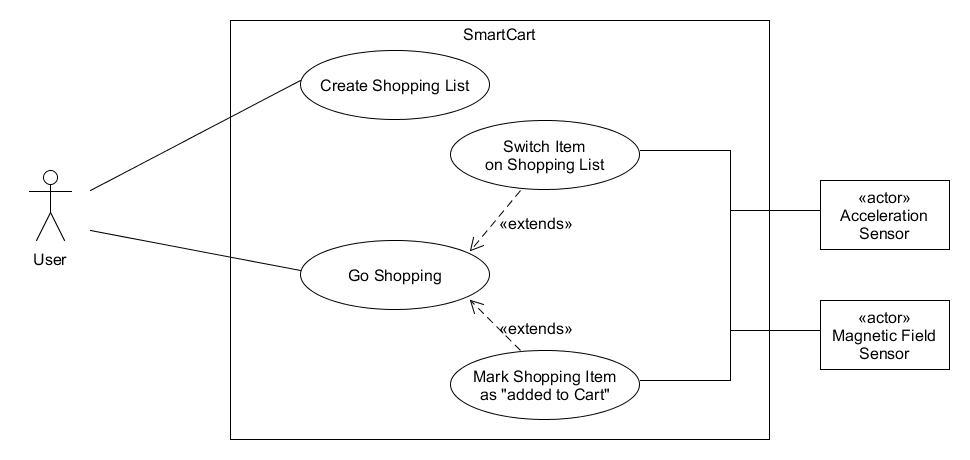
\includegraphics[width=\textwidth]{res/sa/useCaseDiagram.png}
\caption{Overview of the System's Use Cases}
\label{fig:UseCases}
\end{figure}

\subsection{Relations between the captured Gestures
and the used Sensors}

\label{sect:dataModel}
Figure \ref{fig:DataModel} shows a model of how the smartphone, the sensors and
the gestures that should be recognized are related to each other. The
acceleration sensor provides information about the smartphone's speed-up along
its coordinate axes. In the most cases, these axes are not aligned with the
standard x-y-z axes because of the smartphones orientation. Since the
orientation affects the measured acceleration values, it has to be taken into
account when recognizing the user's gestures.

\begin{figure}
\centering
\captionsetup{justification=centering}
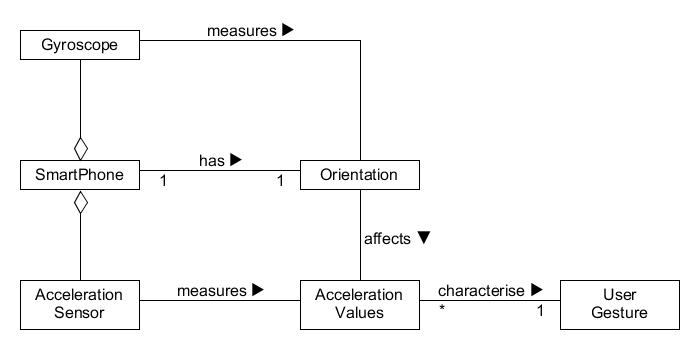
\includegraphics[width=\textwidth]{res/sa/UserGestureDataModel.png}
\caption{Data Model of the User Gestures to recognize}
\label{fig:DataModel}
\end{figure}

\subsection{Application Context}
The context of the application can be retrieved from figure \ref{fig:context}.
The inputs are the values of the accelerometer $a_x$, $a_y$ and $a_z$ as well as
the angles $azimuth$, $pitch$ and $roll$ that determine the smartphones
orientation. The current state and any other information of the application are
visualized on the smartphone's display.

\begin{figure}
\centering
\captionsetup{justification=centering}
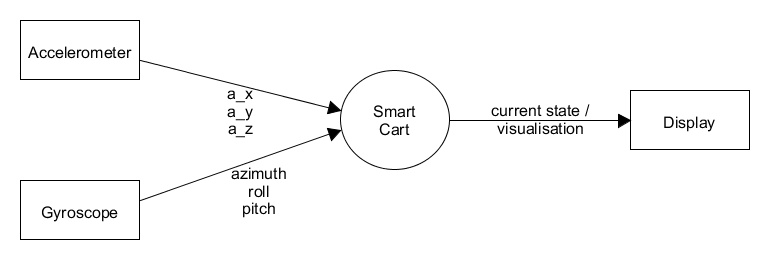
\includegraphics[width=\textwidth]{res/sa/ContextDiagram.png}
\caption{Context of the Application to develop}
\label{fig:context}
\end{figure}


\subsection{Finite State Machine}
hier war noch nicht sicher welche gesten �berhaupt verwendet werden und bla bla
bla (vllt einfach ner murks state machine machen weil die vom dio der letzte
rotz ist und absolut flasch)
\subsubsection{First State Machine}
auf jedenfall zuerst diese kackendreck state machin richtig falsch machen aber
dennoch wenigstens halbwegs sinnvoll
\begin{figure}
\centering
\captionsetup{justification=centering}
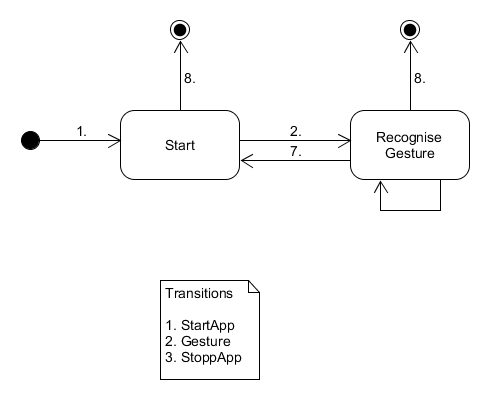
\includegraphics[width=\textwidth]{res/sa/PresentationStateMachineOld.png}
\caption{First Finite State Machine}
\label{fig:first state machine}
\end{figure}

\subsubsection{Evolutioned State Machine}
auch diese self �berg�nge erkl�ren\ldots also alles darf passieren uznd er
bleibt in diesem state

\textbf{Statemachine nochmals anpsassen weil weniger states inzwischen haben.
Urhzeigersinn = abhaken, gegen=n�chstes item. in start kann die liste angelegt
werden usw und wenn mer nach rechts swiped ist das start shopping}

\begin{figure}
\centering
\captionsetup{justification=centering}
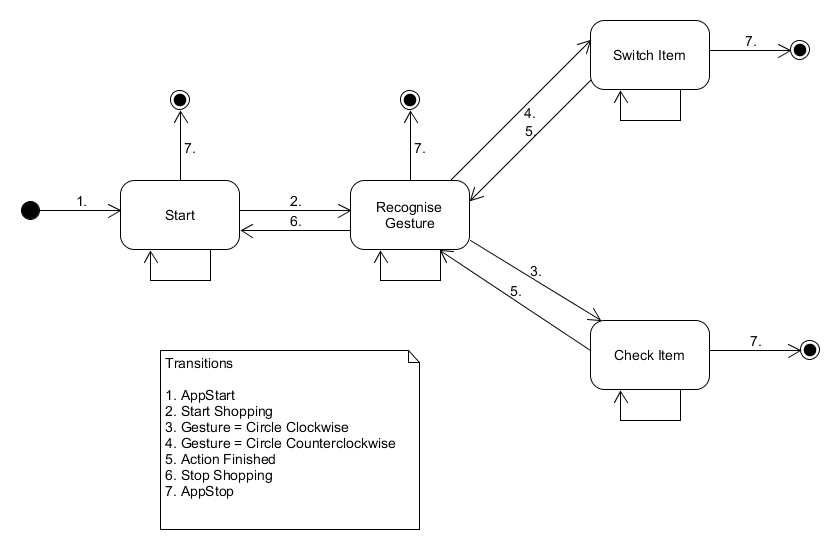
\includegraphics[width=\textwidth]{res/sa/PresentationStateMachineNew.png}
\caption{Evolutioned Finite State Machine}
\label{fig:evo state machine}
\end{figure}


